\section{Basic Idea}
\subsection{Fallacy: LBA-based lifetime prediction}

Current automatic methods predict the lifetime of data based on the update
frequency of LBAs~\cite{AutoStream}.  
For example, AutoStream~\cite{AutoStream} assumes that, if
some LBAs are frequently rewritten by applications, those LBAs hold hot data.
This LBA-based lifetime prediction works poorly on modern applications, where
the majority of new data are written in an append-only manner.  To understand
the correlation between LBAs and the lifetime of data under append-only
workloads, we analyzed the write pattern of RocksDB~\cite{RocksDB}, which is a
popular key-value store based on the LSM-tree algorithm~\cite{LSM}.

Fig.~\ref{fig:lba_lifetime}(a) shows the lifetime distribution of data
according to LBAs. Here, the lifetime of data is defined to be 
the number of write requests between when the data is written 
and when the data is invalidated by an overwrite or a TRIM command. 
%an elapsed time (unit: $\mu$sec) from when it is newly written to a certain LBA to when it is
%invalidated by an overwrite or a TRIM command. 
As shown in
Fig.~\ref{fig:lba_lifetime}(a), there is no strong correlation between the
lifetime and LBAs -- all the data have very different lifetimes, regardless of
their LBA numbers. We also analyzed 
how the lifetimes of LBAs change under some predictable patterns over times 
although the overall lifetime distribution of LBAs shows large variances.
Fig.~\ref{fig:lba_lifetime}(a) shows a scatter plot of data lifetimes over the logical time 
(in the number of write requests) for a 1-MB chunk with \textcolor{red}{2048 LBAs (FIXME: is it right?)}. 
Over the logical time, the lifetime of data written to the chunk 
varies in an unpredictable fashion.  
For example, at the logical time 10, the lifetime was 1 but it increases about 
2.6 million around the logical time 450 
followed by a rapid drop around the logical time 600. 

Our investigation strongly suggests that  under append-only
workloads, LBAs couldn't be a useful 
indicator to decide
the hotness or lifetime of data.

\begin{figure}[t]
	\vspace{-10pt}
	\centering
	\subfloat[Lifetime patterns over LBAs]{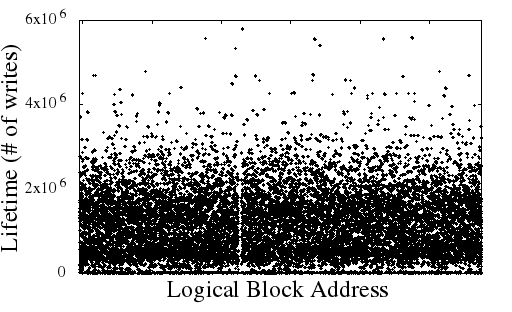
\includegraphics[width=0.25\textwidth]{figure/lba_lifetime2}}  % data from 0/03031641
	\subfloat[Lifetime patterns over time]{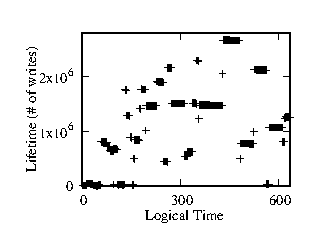
\includegraphics[width=0.22\textwidth]{figure/lifetime_in_chunk2}}
	%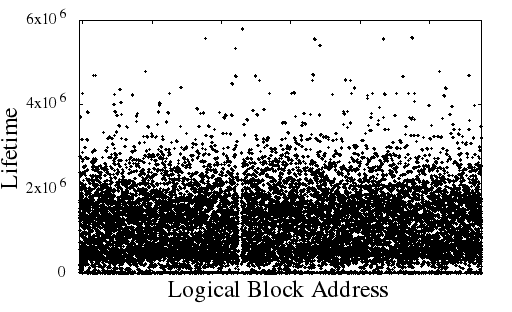
\includegraphics[width=0.9\linewidth]{figure/lba_lifetime} 
	\vspace{-10pt}
	\caption{
		Data lifetime distributions over varying LBAs and logical times.
		\textcolor{red}{(TODO:) it would be good to include same graphs with
		in-place update workloads;}}
		\label{fig:lba_lifetime}
	\vspace{-15pt}
\end{figure}

\vspace{-5pt}
\subsection{Program context as a lifetime predictor}
In order to separate data with different lifetimes, the key requirement is to devise 
a means with which {\it different I/O contexts} can be effectively distinguished.  
For example, LBAs played such a role fairly well for update workloads.  
However, they do not work well for append-only workloads because 
they do not convey the context of I/O operations any more.  

In developing PCStream, we started from a simple question: 
how can we extract I/O context from an application? 
For example, in RocksDB, logging, flushing and compaction can be regarded
as different I/O contexts.
RocksDB appends write-ahead logs to storage to ensure data
persistence.  Those logs have short lifetimes because they are quickly deleted
after original data are persistently stored.
The flush module (which materializes the content of a memtable in
DRAM, called an L0 table, to an L1 table in the storage) generates data
with relatively short lifetimes. This is because an L1 table will be flushed to
an L2 table and be removed in the near future. Conversely, a compaction module
writes long-lived data that are unlikely to be removed for a long time.

The above observation implies that, if we are able to know the detailed
behaviors of append-only applications, data with different lifetimes can be
isolated in separate streams in an SSD. As mentioned before, a common
solution~\cite{MultiStream} to realizing this is manually modify an application
code so that each module assigns a unique stream ID to data it generates.
However, owing to considerable implementation efforts required to modify
individual applications, this approach is not widely used in practice.

In this paper, we claim that a program context (PC) is a useful tool that delivers
the information of data lifetimes to the storage side without modifying
application code manually. A PC is calculated at runtime by
summing the values of program counters that are identified along function-call
paths of an application. Logging, flushing, and compaction are invoked through
different function-call paths. Thus, by leveraging PCs, we are
able to identify software modules that generate specific write streams. Note
that using PCs to identify characteristics of data is not new.
Ha \textit{et al.} proposed a way of separating hot-cold data by referring to
PCs~\cite{PCHa}. This work, however, was not designed for
append-only applications and didn't take into account the use of a multi-stream
feature of a modern SSD.

\begin{figure}[!t]
\centering
\vspace{-10pt}
\hspace{1pt}
\subfloat[\texttt{manual}: log]{
\includegraphics[width=0.23\textwidth]{figure/type_1b}} % data from 4/03031953 
\subfloat[\texttt{automatic}: log]{
\includegraphics[width=0.23\textwidth]{figure/pcID_2b}}
\hfill
\vspace{-10pt}
\subfloat[\texttt{manual}: flush] {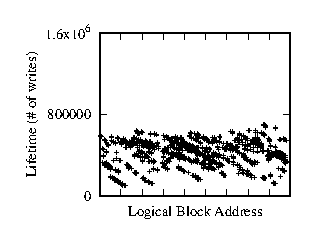
\includegraphics[width=0.23\textwidth]{figure/type_3b}}
\subfloat[\texttt{automatic}: flush]{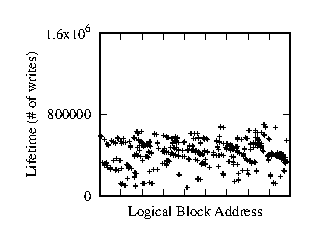
\includegraphics[width=0.23\textwidth]{figure/pcID_3b}}
\caption{Data lifetime distributions of different PCs.} 
\label{fig:types_and_PCs}
\vspace{-15pt}
\end{figure}

In order to confirm our hypothesis that PCs could provide enough information to
recognize the lifetimes of data based on detailed application behaviors, we
conducted experiments using RocksDB, comparing the accuracy of lifetime
prediction of two different methods: 1) when the type of data streams is
manually identified by modifying the code (\texttt{manual}) and 2) when the
stream type is automatically tagged by PCs (\texttt{automatic}).
Fig.~\ref{fig:types_and_PCs} compares the lifetime distributions of data
separated by \texttt{manual} and \texttt{automatic}.
Figs.~\ref{fig:types_and_PCs}(a) and (b) represent how well the two methods
identify log data written by RocksDB. The \texttt{automatic} method with PCs
shows high accuracy to detect log data with short lifetimes, which is
comparable to \texttt{manual}. Similarly, Figs.~\ref{fig:types_and_PCs}(c) and
(d) shows the accuracy of identifying data written by the flush module of
RocksDB.  As expected, these two graphs have the similar lifetime patterns,
which proves that PCs can be a good lifetime hint.


